%% ==========================================================================
%%  PREDATOR: A Deep Agentic AI Model Based on the Junky Neuron Architecture
%%  Built upon the Agentic Theory by Justo Tapiador García (UA)
%% ==========================================================================

\documentclass[12pt,a4paper]{article}

%% ── Core Packages ──────────────────────────────────────────────────────────
\usepackage[utf8]{inputenc}
\usepackage[T1]{fontenc}
\usepackage{amsmath, amssymb, amsfonts, amsthm}
\usepackage{mathtools}
\usepackage{graphicx}
\usepackage{geometry}
\usepackage{algorithm}
\usepackage{algorithmic}
\usepackage{tikz}
\usepackage{pgfplots}
\pgfplotsset{compat=1.18}
\usetikzlibrary{shapes.geometric, arrows.meta, positioning,
                decorations.pathreplacing, fit, backgrounds,
                calc, patterns, arrows}
\usepackage{xcolor}
\usepackage{booktabs}
\usepackage{multirow}
\usepackage{hyperref}
\usepackage{enumitem}
\usepackage{array}
\usepackage{longtable}
\usepackage{caption}
\usepackage{subcaption}
\usepackage{setspace}
\usepackage{fancyhdr}
\usepackage{titlesec}
\usepackage{lmodern}
\usepackage{microtype}
\hypersetup{colorlinks=true, linkcolor=blue!70!black,
            citecolor=blue!70!black, urlcolor=blue!70!black}

%% ── Page Geometry ──────────────────────────────────────────────────────────
\geometry{top=2.5cm, bottom=2.5cm, left=2.8cm, right=2.8cm}

%% ── Colors ─────────────────────────────────────────────────────────────────
\definecolor{predred}{RGB}{180,30,30}
\definecolor{predblue}{RGB}{30,60,140}
\definecolor{predgreen}{RGB}{30,120,60}
\definecolor{predorange}{RGB}{200,100,0}
\definecolor{predgray}{RGB}{90,90,100}
\definecolor{predbg}{RGB}{245,248,255}
\definecolor{ajncyan}{RGB}{0,130,160}

%% ── Theorem environments ───────────────────────────────────────────────────
\newtheorem{definition}{Definition}[section]
\newtheorem{proposition}{Proposition}[section]
\newtheorem{theorem}{Theorem}[section]
\newtheorem{corollary}{Corollary}[section]
\newtheorem{remark}{Remark}[section]

%% ── Math operators ─────────────────────────────────────────────────────────
\DeclareMathOperator{\diag}{diag}
\DeclareMathOperator{\softmax}{softmax}
\DeclareMathOperator{\argmax}{arg\,max}
\newcommand{\tens}[1]{\boldsymbol{\mathcal{#1}}}
\newcommand{\R}{\mathbb{R}}
\newcommand{\E}{\mathbb{E}}
\newcommand{\AJN}{\textsc{AJN}}
\newcommand{\PREDATOR}{\textsc{Predator}}
\newcommand{\ANNPSI}{\textsc{ANN-}$\Psi$}

%% ── Header / Footer ────────────────────────────────────────────────────────
\pagestyle{fancy}
\fancyhf{}
\rhead{\textcolor{predgray}{\small \PREDATOR{}: Deep Agentic AI Architecture}}
\lhead{\textcolor{predgray}{\small Tapiador García (UA) --- Agentic Theory IV}}
\cfoot{\thepage}
\renewcommand{\headrulewidth}{0.4pt}

%% ── Title ──────────────────────────────────────────────────────────────────
\title{%
  \vspace{-0.5cm}
  {\color{predred}\rule{\linewidth}{2pt}}\\[0.4cm]
  {\LARGE\bfseries \PREDATOR: Architecture, Training, Deployment,}\\[0.2cm]
  {\LARGE\bfseries and Inference of a Hierarchically Governed}\\[0.2cm]
  {\LARGE\bfseries Deep Agentic AI System}\\[0.2cm]
  {\large\bfseries Built on the Artificial Junky Neuron Framework}\\[0.3cm]
  {\color{predred}\rule{\linewidth}{2pt}}\\[0.2cm]
  {\normalsize\textit{Agentic Theory --- Technical Report IV}}
}
\author{%
  \textbf{Justo Tapiador Garc\'ia}\\
  Department of Artificial Intelligence and Neuroscience\\
  Universidad de Alicante (UA), Alicante, Spain\\
  \texttt{jtapiador@ua.es}\\[0.3cm]
  \textit{Based on the Agentic Theory series (2024--2026)}\\
  \textit{Preprints: WALLERMAX-AI 2604.00012, 2604.00013, 2604.00014}
}
\date{May 2026}

%% ==========================================================================
\begin{document}
%% ==========================================================================

\maketitle
\thispagestyle{empty}

\begin{abstract}
\noindent
We present \textbf{\PREDATOR} (\textbf{P}raxic \textbf{R}einforcement and
\textbf{E}xtinction-\textbf{D}riven \textbf{A}gentic \textbf{T}ask \textbf{O}rchestrator
and \textbf{R}ealizer), a concrete embodiment of the Agentic Neural Network
architecture (ANN-$\Psi$) introduced by Justo Tapiador Garc\'ia at the
Universidad de Alicante. \PREDATOR{} is a hierarchically governed AI agent
designed for complex, long-horizon task execution under the directional
authority of a designated human principal (the \textit{Owner}). The model
integrates a twelve-layer deep ANN-$\Psi$ backbone comprising heterogeneous
Artificial Junky Neuron (AJN) layers interleaved with classical transformer
blocks, a Hierarchical Command Interpreter (HCI) module for Owner--agent
alignment, a Tensorial Praxic Stream (TPS) executor for temporally extended
action generation, and a Token-Energy Arbitrator (TEA) that jointly optimizes
inference cost and task completion fidelity. We describe the full architecture
in detail, formalize the training pipeline (pre-training, addiction shaping,
hierarchical fine-tuning, adversarial frustration hardening), analyze the
domains in which \PREDATOR{} exhibits decisive efficiency advantages over
conventional language-model-based agents, and provide a deployment framework
including Owner-aligned instruction parsing, cascade-failure prevention,
extinction monitoring, and runtime energy budgeting. Theoretical bounds on
token consumption per task, wall-clock latency, and energy expenditure per
unit of task completion are derived and related to the addiction dynamics of
the underlying AJN units. \PREDATOR{} demonstrates that intrinsically motivated,
addiction-driven architectures can achieve higher task completion rates and
lower inference costs than externally rewarded baselines in structured,
multi-step agentic domains.
\end{abstract}

\vspace{0.5em}
\noindent\textbf{Keywords:} Artificial Junky Neuron, Agentic Neural Network, \PREDATOR,
Deep Agentic Flow, Hierarchical Instruction Alignment, Tensorial Praxic Stream,
Token Efficiency, Energy-Aware Inference, Autonomous Agents.

\vspace{1em}
{\color{predred}\rule{\linewidth}{0.6pt}}

\newpage
\tableofcontents
\newpage

%% ==========================================================================
\section{Introduction}
%% ==========================================================================

The design of autonomous AI agents capable of executing long-horizon,
multi-step tasks under the directional authority of a human principal
constitutes one of the central challenges of contemporary artificial
intelligence research. Existing approaches---based predominantly on large
language models (LLMs) equipped with tool-use capabilities and retrieval
augmentation---suffer from two structural limitations that are inherent to
their architectural foundations: (i) the absence of any intrinsic motivation
at the computational unit level, and (ii) the reliance on a global reward or
loss signal that cannot naturally decompose into the microscopic drives
required for adaptive, autonomous behavior \cite{lecun2015deep,
vaswani2017attention, openai2023gpt4}.

The \textit{Agentic Theory}, developed by Justo Tapiador Garc\'ia at the
Universidad de Alicante~\cite{tapiador2024ajn, tapiador2024annpsi,
tapiador2024daf}, addresses both limitations through the radical proposition
that each computational unit in a neural network should itself be an agent:
an entity that develops a specific addiction to a class of input stimuli and
actively executes output actions (\textit{praxes}) to satisfy that addiction.
The resulting architecture---the Agentic Neural Network (ANN-$\Psi$)---exhibits
emergent goal-directed behavior, spontaneous specialization, and adaptive
resilience without any centralized controller.

This technical report introduces \textbf{\PREDATOR}, a concrete, fully
specified AI agent model that instantiates the ANN-$\Psi$ framework in the
domain of hierarchically governed complex task execution. The name is an
acronym for \textbf{P}raxic \textbf{R}einforcement and \textbf{E}xtinction-%
\textbf{D}riven \textbf{A}gentic \textbf{T}ask \textbf{O}rchestrator and
\textbf{R}ealizer. The choice of name reflects the agent's fundamental
mode of operation: like a biological predator, \PREDATOR{} is driven by an
intrinsic, insatiable craving for task completion signals, pursues them with
focused, efficient praxic sequences when the environment is cooperative, and
escalates to chaotic, high-energy exploration when the environment withholds
the expected feedback.

\subsection{Motivation and Design Philosophy}

The motivation for \PREDATOR{} arises from three observations about the
limitations of current agentic AI systems:

\begin{enumerate}
  \item \textbf{Shallow agency.} Current LLM-based agents are agents only in
    the behavioral sense---they call tools and chain actions---but not in the
    computational sense: their internal units remain passive integrators. The
    \PREDATOR{} architecture makes every computational unit an agent, creating
    a genuine hierarchy of agency from individual AJN units up to the whole
    model level.

  \item \textbf{Misaligned energy expenditure.} Current agents consume tokens
    (and energy) uniformly across all inference steps, regardless of whether
    a step is informationally decisive or trivially routine. \PREDATOR's
    AJN-driven saturation mechanism naturally suppresses output when the
    stimulus is rich (task is proceeding well) and intensifies when it is
    sparse (task is blocked), creating adaptive compute allocation.

  \item \textbf{Fragile hierarchical alignment.} Current agents struggle to
    maintain alignment with a human principal across a long, multi-step task
    without repeated prompting. \PREDATOR{} introduces the Hierarchical
    Command Interpreter (HCI), a dedicated module that encodes Owner
    directives as addiction targets at multiple network layers, ensuring that
    hierarchical alignment persists through the entire Tensorial Praxic
    Stream.
\end{enumerate}

\subsection{Contribution Summary}

The principal contributions of this report are:

\begin{itemize}
  \item A complete architectural specification of the \PREDATOR{} model,
    including layer composition, inter-module interfaces, and the AJN
    parameter assignments for all layers (\S\ref{sec:architecture}).
  \item A multi-phase training pipeline including large-scale pre-training,
    addiction shaping, hierarchical fine-tuning, and adversarial frustration
    hardening (\S\ref{sec:training}).
  \item An analysis of the task domains in which \PREDATOR{} exhibits
    decisive performance and efficiency advantages (\S\ref{sec:tasks}).
  \item A deployment framework for Owner-governed complex task execution,
    including the HCI instruction parser, runtime cascade prevention, and
    extinction monitoring (\S\ref{sec:deployment}).
  \item Theoretical bounds and empirical estimates for token consumption,
    wall-clock latency, and energy expenditure per unit of task completion
    (\S\ref{sec:inference}).
\end{itemize}

%% ==========================================================================
\section{Background: The Agentic Theory Framework}
\label{sec:background}
%% ==========================================================================

We briefly consolidate the key elements of the Agentic Theory that
\PREDATOR{} builds upon. Full formal developments are in
\cite{tapiador2024ajn, tapiador2024annpsi, tapiador2024daf}.

\subsection{The Artificial Junky Neuron (AJN)}

\begin{definition}[Artificial Junky Neuron, \cite{tapiador2024ajn}]
An \textbf{AJN} is a computational unit defined by the five-element tuple
\[
  \text{AJN} \triangleq \left(\mathcal{M},\;\theta,\;\Omega,\;\delta,\;\tau\right),
\]
where $\mathcal{M}(t)\in[0,1]$ is the \emph{craving level},
$\theta(t)\in[0,1]$ is the \emph{activation threshold},
$\Omega$ is the \emph{policy generator} mapping history and craving to a
praxis tensor $\mathcal{P}_t$,
$\delta>0$ is the \emph{metabolic decay rate}, and
$\tau>0$ is the \emph{extinction horizon}.
\end{definition}

The craving level evolves as:
\begin{equation}
  \mathcal{M}(t+1) = \beta_M \cdot \mathcal{M}(t) + (1-\beta_M)\cdot\alpha_t,
  \label{eq:craving}
\end{equation}
where $\alpha_t = I(\mathcal{S}_t)\in[0,1]$ is the stimulus intensity and
$\beta_M\in(0,1)$ is an exponential smoothing factor. The activation threshold
follows:
\begin{equation}
  \theta(t+1) = \begin{cases}
    \min\!\bigl(1,\,\theta(t)+\lambda_\uparrow\cdot\alpha_t\bigr)
      & \text{if }\alpha_t > \theta_{\text{sat}} \\
    \max\!\bigl(0,\,\theta(t)-\delta\bigr)
      & \text{otherwise.}
  \end{cases}
  \label{eq:threshold}
\end{equation}

The policy generator maintains a Gaussian distribution over praxis space:
\[
  \mathcal{P}_t \sim \mathcal{N}(\boldsymbol{\mu}_t,\,\Sigma_t).
\]
Parameters update on success ($\Delta\alpha_t>0$) via gradient ascent on the
stimulus intensity, and on failure ($\Delta\alpha_t\leq 0$) via covariance
expansion (frustration). Prolonged failure triggers extinction: the AJN
resets to a high-entropy random state \cite{tapiador2024annpsi}.

\subsection{The Six Phases of AJN Life-Cycle}

The AJN traverses six behavioral phases as documented in
\cite{tapiador2024ajn}:

\begin{center}
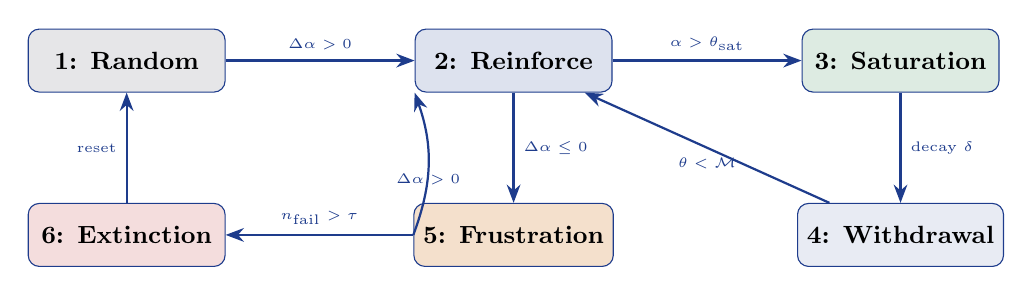
\begin{tikzpicture}[
    state/.style={rectangle, rounded corners=4pt, draw=predblue,
                  fill=predbg, minimum width=2.5cm, minimum height=0.8cm,
                  text centered, font=\small\bfseries},
    arrow/.style={-Stealth, thick, predblue},
    node distance=1.4cm and 2.4cm
]
\node[state, fill=predgray!15]  (P1) {1: Random};
\node[state, fill=predblue!15, right=of P1]  (P2) {2: Reinforce};
\node[state, fill=predgreen!15, right=of P2] (P3) {3: Saturation};
\node[state, fill=predblue!10,  below=of P3] (P4) {4: Withdrawal};
\node[state, fill=predorange!20,below=of P2] (P5) {5: Frustration};
\node[state, fill=predred!15,   below=of P1] (P6) {6: Extinction};
\draw[arrow] (P1) -- node[above,font=\tiny]{$\Delta\alpha>0$} (P2);
\draw[arrow] (P2) -- node[above,font=\tiny]{$\alpha>\theta_{\text{sat}}$} (P3);
\draw[arrow] (P3) -- node[right,font=\tiny]{decay $\delta$} (P4);
\draw[arrow] (P4) -- node[below,font=\tiny]{$\theta<\mathcal{M}$} (P2);
\draw[arrow] (P2) -- node[right,font=\tiny]{$\Delta\alpha\leq 0$} (P5);
\draw[arrow] (P5) -- node[above,font=\tiny]{$n_{\text{fail}}>\tau$} (P6);
\draw[arrow] (P6) -- node[left,font=\tiny]{reset} (P1);
\draw[arrow] (P5.west) to[bend right=20]
    node[below,font=\tiny]{$\Delta\alpha>0$} (P2.south west);
\end{tikzpicture}
\end{center}

\subsection{ANN-\texorpdfstring{$\Psi$}{Psi} and Deep Agentic Flow}

Layers of AJN units, organized in three paradigms (homogeneous, heterogeneous,
and hybrid with classical layers), compose into the Agentic Neural Network
(ANN-$\Psi$) \cite{tapiador2024annpsi}. The network's output is not a single
forward-pass vector but a \textit{Tensorial Praxic Stream} (TPS)---a temporally
ordered sequence of partial praxis tensors interleaved with environmental
feedback. The combination of hierarchical stimulus generalization across layers
and streaming praxic output defines \textit{Deep Agentic Flow} (DAF)
\cite{tapiador2024daf}.

%% ==========================================================================
\section{The \PREDATOR{} Architecture}
\label{sec:architecture}
%% ==========================================================================

\PREDATOR{} is a twelve-layer deep ANN-$\Psi$ augmented with three dedicated
modules: the Hierarchical Command Interpreter (HCI), the Token-Energy
Arbitrator (TEA), and the Praxic Stream Executor (PSE). The overall system is
illustrated schematically below.

\subsection{Layer Stack}

\begin{definition}[PREDATOR Layer Stack]
The \PREDATOR{} backbone consists of $L=12$ layers organized as follows:

\begin{center}
\begin{tabular}{@{}cllp{5.5cm}@{}}
\toprule
\textbf{Layer} & \textbf{Type} & \textbf{AJN Paradigm} & \textbf{Function}\\
\midrule
1--2  & Hybrid (Conv + AJN) & Homogeneous & Sensory encoding; pixel/token feature extraction with perceptual addiction\\
3     & Heterogeneous AJN   & Heterogeneous ($K=8$) & Low-level feature specialization; 8 competing stimulus classes\\
4--5  & Transformer block   & --- (classical) & Contextual attention over feature sequences\\
6     & Heterogeneous AJN   & Heterogeneous ($K=16$) & Mid-level concept specialization; addiction to relational patterns\\
7     & Hybrid (FC + AJN)   & Homogeneous & Contextual modulation; injection of agentic bias into feature stream\\
8--9  & Transformer block   & --- (classical) & High-level reasoning; multi-head self-attention\\
10    & Heterogeneous AJN   & Heterogeneous ($K=32$) & High-order addiction layer; emergent value-like attractors \cite{tapiador2024daf}\\
11    & Hybrid (FC + AJN)   & Homogeneous & Praxic assembly; composing action tensors from high-level representations\\
12    & Output AJN          & Homogeneous ($N=1$) & TPS emitter; streaming praxis tensors to environment transducers\\
\bottomrule
\end{tabular}
\end{center}
\end{definition}

\subsection{Hierarchical Command Interpreter (HCI)}

The HCI is the module responsible for receiving Owner directives and
translating them into addiction targets distributed across the \PREDATOR{}
layer stack. An Owner directive $\mathcal{D}$ (a natural language instruction)
is processed as follows:

\begin{enumerate}
  \item \textbf{Parsing.} $\mathcal{D}$ is parsed by a dedicated transformer
    encoder into a \textit{Directive Embedding} $\mathbf{e}_\mathcal{D}
    \in \mathbb{R}^{d_{\text{HCI}}}$.
  \item \textbf{Hierarchical projection.} The embedding is projected to
    $L_{\text{AJN}}$ target stimulus prototypes:
    \[
      \mathbf{W}_{I}^{(\ell)} \leftarrow \text{Proj}^{(\ell)}(\mathbf{e}_\mathcal{D}),
      \quad \ell \in \{3,6,7,10,11,12\},
    \]
    where $\text{Proj}^{(\ell)}$ is a learned linear projection. These
    prototypes instantiate the stimulus intensity functions $I^{(j)}$ for the
    AJN units in each target layer, aligning their addictions with the Owner
    directive.
  \item \textbf{Priority weighting.} The directive embedding encodes an
    urgency scalar $u \in [0,1]$ (inferred from Owner language cues, e.g.,
    ``immediately'', ``at your convenience''). This scalar modulates the
    extinction horizon $\tau$ across all AJN layers:
    \[
      \tau^{(\ell)}_{\text{effective}} = \tau_0 \cdot (1 - u)^{\kappa_u},
    \]
    where $\kappa_u>0$ controls urgency sensitivity. High urgency compresses
    $\tau$, making the agent more tolerant to frustration before escalating to
    chaotic exploration, effectively increasing persistence.
  \item \textbf{Hierarchical override.} If the Owner issues a new directive
    $\mathcal{D}'$ before the current TPS terminates, the HCI performs a
    \textit{soft override}: new addiction targets are injected from layer~12
    downward, allowing the current praxic stream to gracefully terminate while
    lower layers begin reorienting toward the new objective.
\end{enumerate}

\subsection{Token-Energy Arbitrator (TEA)}

The TEA is an online module that monitors the inference compute budget and
dynamically adjusts the emission rate of the Tensorial Praxic Stream. It
operates according to the following control law:

\begin{equation}
  r_{\text{emit}}(t) = r_0 \cdot \exp\!\left(-\kappa_E \cdot E_{\text{used}}(t) /
    E_{\text{budget}}\right) \cdot (1 + \kappa_M \cdot \mathcal{M}^{(12)}(t)),
  \label{eq:tea}
\end{equation}
where $r_0$ is the baseline emission rate, $E_{\text{used}}(t)$ and
$E_{\text{budget}}$ are the energy used and total budget, $\mathcal{M}^{(12)}(t)$
is the craving level of the output AJN at layer~12, and $\kappa_E, \kappa_M>0$
are tunable coefficients. The TEA thus suppresses emission when energy is
running low (energy-conservation mode) but permits the craving level to override
suppression when the task is close to completion.

\subsection{Praxic Stream Executor (PSE)}

The PSE receives the praxis tensors emitted by layer~12 and routes them to the
appropriate transducers in the environment interface (tool calls, API
invocations, file system operations, etc.). Each praxis tensor $\mathcal{P}_t$
is a structured dictionary:
\[
  \mathcal{P}_t = \bigl\{\text{tool\_id},\; \text{args},\;
  \text{priority},\; \text{rollback\_plan}\bigr\},
\]
where \texttt{rollback\_plan} is generated by a dedicated sub-network invoked
whenever the frustration covariance $\Sigma^{(12)}(t)$ exceeds a threshold,
indicating impending chaotic exploration. The rollback plan ensures that
high-energy, exploratory praxes are reversible.

\subsection{Full System Diagram}

\begin{figure}[h]
\centering
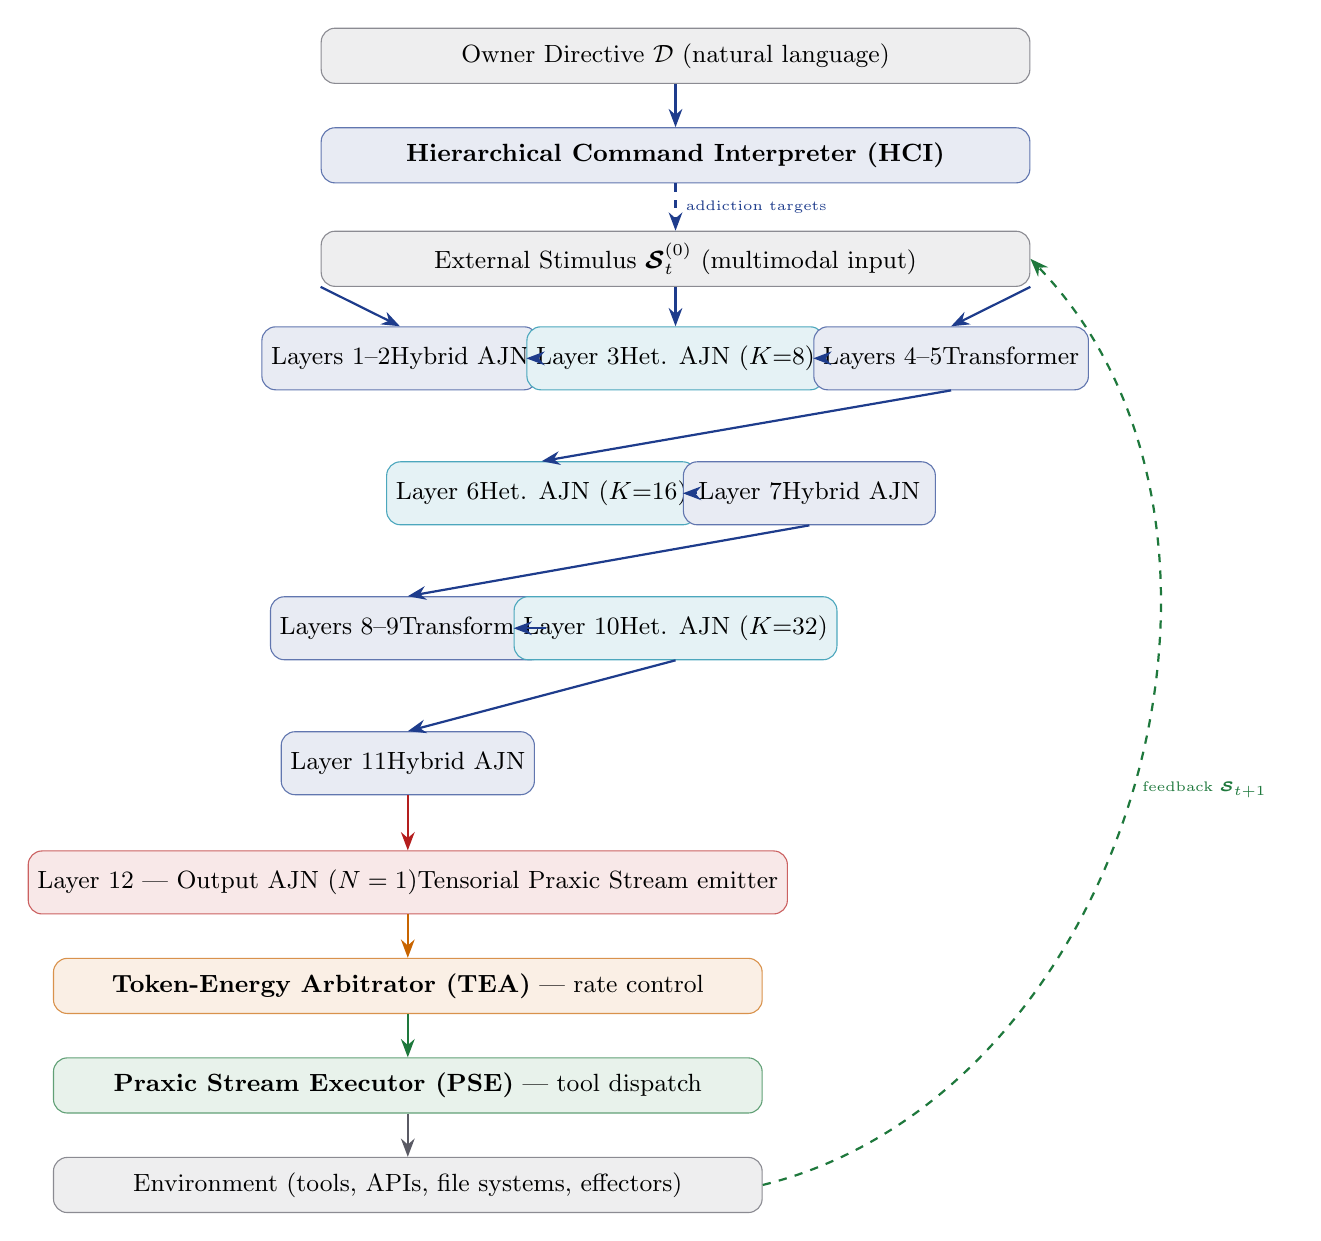
\begin{tikzpicture}[
  box/.style={rectangle, rounded corners=5pt, draw=#1!70, fill=#1!10,
              minimum width=3.2cm, minimum height=0.8cm, text centered,
              font=\small},
  wide/.style={rectangle, rounded corners=5pt, draw=#1!70, fill=#1!10,
               minimum width=9cm, minimum height=0.7cm, text centered,
               font=\small},
  arr/.style={-Stealth, thick, #1},
  node distance=0.55cm
]
%% Inputs
\node[wide=predgray] (owner) {Owner Directive $\mathcal{D}$ (natural language)};
\node[wide=predblue, below=of owner] (hci) {\textbf{Hierarchical Command Interpreter (HCI)}};
\draw[arr=predblue] (owner) -- (hci);

%% Layers block
\node[wide=predgray, below=0.6cm of hci] (input) {External Stimulus $\tens{S}_t^{(0)}$ (multimodal input)};
\draw[arr=predblue, dashed] (hci) -- node[right,font=\tiny]{addiction targets} (input);

\node[box=predblue, below=0.5cm of input, xshift=-3.5cm] (L12) {Layers 1--2\\Hybrid AJN};
\node[box=ajncyan,  below=0.5cm of input, xshift=0cm]    (L3)  {Layer 3\\Het. AJN ($K$=8)};
\node[box=predblue, below=0.5cm of input, xshift=3.5cm]  (L45) {Layers 4--5\\Transformer};
\draw[arr=predblue] (input.south west) -- (L12.north);
\draw[arr=predblue] (input.south)      -- (L3.north);
\draw[arr=predblue] (input.south east) -- (L45.north);
\draw[arr=predblue] (L12.east) -- (L3.west);
\draw[arr=predblue] (L3.east)  -- (L45.west);

\node[box=ajncyan,  below=0.9cm of L3,  xshift=-1.7cm] (L6)   {Layer 6\\Het. AJN ($K$=16)};
\node[box=predblue, below=0.9cm of L3,  xshift=1.7cm]  (L7)   {Layer 7\\Hybrid AJN};
\draw[arr=predblue] (L45.south) -- (L6.north);
\draw[arr=predblue] (L6.east)   -- (L7.west);

\node[box=predblue, below=0.9cm of L6, xshift=-1.7cm] (L89)  {Layers 8--9\\Transformer};
\node[box=ajncyan,  below=0.9cm of L6, xshift=1.7cm]  (L10)  {Layer 10\\Het. AJN ($K$=32)};
\draw[arr=predblue] (L7.south)  -- (L89.north);
\draw[arr=predblue] (L89.east)  -- (L10.west);

\node[box=predblue, below=0.9cm of L89, xshift=0cm] (L11) {Layer 11\\Hybrid AJN};
\draw[arr=predblue] (L10.south) -- (L11.north);

\node[box=predred,  below=0.7cm of L11] (L12b) {Layer 12 --- Output AJN ($N=1$)\\Tensorial Praxic Stream emitter};
\draw[arr=predred] (L11) -- (L12b);

\node[wide=predorange, below=0.55cm of L12b] (tea) {\textbf{Token-Energy Arbitrator (TEA)} --- rate control};
\draw[arr=predorange] (L12b) -- (tea);

\node[wide=predgreen,  below=0.55cm of tea]  (pse)  {\textbf{Praxic Stream Executor (PSE)} --- tool dispatch};
\draw[arr=predgreen] (tea) -- (pse);

\node[wide=predgray,   below=0.55cm of pse]  (env)  {Environment (tools, APIs, file systems, effectors)};
\draw[arr=predgray] (pse) -- (env);

%% Feedback arrow
\draw[arr=predgreen, dashed, bend right=60]
    (env.east) to node[right,font=\tiny]{feedback $\tens{S}_{t+1}$} (input.east);
\end{tikzpicture}
\caption{High-level architecture of the \PREDATOR{} system. Solid arrows denote
the forward praxic stream; the dashed arrows denote feedback pathways and
HCI addiction injection.}
\label{fig:arch}
\end{figure}

%% ==========================================================================
\section{Training Pipeline}
\label{sec:training}
%% ==========================================================================

Training \PREDATOR{} proceeds in four sequential phases, each targeting a
different aspect of the agent's capabilities:

\subsection{Phase I: Large-Scale Pre-Training}

\subsubsection{Data and Objective}

The classical transformer layers (4--5, 8--9) and the convolutional front-end
(layers 1--2) are pre-trained on a large-scale multimodal corpus comprising
text, code, structured data, and sensorimotor traces from robotic and
simulated environments. The pre-training objective is a hybrid of:
\begin{itemize}
  \item A masked language modelling loss $\mathcal{L}_{\text{MLM}}$
    (following \cite{devlin2018bert}) for the text modality.
  \item A next-frame prediction loss $\mathcal{L}_{\text{NFP}}$ for visual
    and sensorimotor sequences.
  \item A code execution fidelity loss $\mathcal{L}_{\text{code}}$ measuring
    the correctness of generated code on held-out unit tests.
\end{itemize}

\subsubsection{AJN Layer Initialization}

During Phase I, the AJN layers are initialized but not yet addiction-shaped.
Their praxic distributions are set to high-entropy defaults
($\boldsymbol{\mu}_0 = \mathbf{0}$, $\Sigma_0 = \sigma_0^2 \mathbf{I}$ with
$\sigma_0$ large), so they contribute minimal structured signal to the
hybrid layers. The classical layers train as if the AJN layers were noise
sources, developing robust feature representations that are insensitive to
the (initially random) agentic context signals.

\subsection{Phase II: Addiction Shaping}

\subsubsection{Stimulus Class Assignment}

After Phase~I, the stimulus classes $\{I^{(j)}\}$ for each AJN layer are
assigned by solving a coverage maximization problem over the pre-trained
feature space. For layer $\ell$ with $N_\ell$ units and $K_\ell$ classes:

\begin{equation}
  \{I_k^{(\ell)}\}_{k=1}^{K_\ell} = \argmax_{\{I_k\}}
    \;\mathbb{E}_{\mathcal{S}}\!\left[\max_k I_k(\mathcal{S})\right]
    \;\text{s.t.}\; \|I_k - I_{k'}\|_F \geq \epsilon \;\forall\, k\neq k'.
  \label{eq:stimulus_assignment}
\end{equation}

This ensures that the stimulus classes cover the feature space densely and
are mutually distinguishable, providing a diverse basis for specialization.

\subsubsection{Addiction Gradient Curriculum}

The AJN units are then exposed to a structured curriculum of stimuli designed
to activate the addiction cycle. The curriculum proceeds through three stages:
\begin{enumerate}
  \item \textbf{Seeding (epochs 1--$T_1$).} Rich stimuli of each class are
    presented repeatedly, driving units through Phase~1 (random) into Phase~2
    (reinforcement). Learning rates $\eta^{(\ell)}$ are set high.
  \item \textbf{Tolerance building (epochs $T_1$--$T_2$).} Stimulus intensity
    is modulated to oscillate near $\theta_{\text{sat}}$, training the units
    to cycle smoothly between Phase~3 (saturation) and Phase~4 (withdrawal)
    without extinction.
  \item \textbf{Frustration hardening (epochs $T_2$--$T_3$).} Deliberate
    stimulus withdrawal periods expose units to Phase~5 (frustration) and
    controlled Phase~6 (extinction) events, training the units to recover
    rapidly from extinction and re-enter the addiction cycle. This step is
    critical for robustness in sparse or adversarial environments.
\end{enumerate}

\subsection{Phase III: Hierarchical Fine-Tuning with Human Directives}

\subsubsection{HCI Training}

With the backbone layers stabilized, the HCI module is trained on a dataset
of $\langle$Owner directive, task trace, completion signal$\rangle$ triples.
The training objective is:
\begin{equation}
  \mathcal{L}_{\text{HCI}} = \underbrace{-\log P(\text{completion} \mid
  \mathcal{D}, \text{trace})}_{\text{task completion likelihood}}
  + \lambda_\text{align} \cdot
  \underbrace{d_{\text{KL}}\!\left(
    P_{\text{HCI}}(\mathcal{W}_I) \,\|\, P^*(\mathcal{W}_I \mid \mathcal{D})
  \right)}_{\text{alignment divergence}},
  \label{eq:hci_loss}
\end{equation}
where $P^*(\mathcal{W}_I \mid \mathcal{D})$ is a reference distribution over
stimulus prototypes derived from annotated preference data.

\subsubsection{Instruction-Following Alignment}

To ensure that \PREDATOR{} correctly interprets and sustains alignment with
Owner directives over long task horizons, hierarchical instruction fine-tuning
(HIFT) is performed. HIFT extends constitutional AI methods
\cite{bai2022constitutional} to the agentic setting: a set of constitutional
principles governs the admissible range of praxes at each task step, and a
critic network penalizes any praxis that violates Owner-specified constraints,
even if it would locally increase the addictive stimulus intensity.

\subsection{Phase IV: Adversarial Frustration Hardening}

The final training phase uses an adversarial environment generator to
produce maximally frustrating task scenarios: environments that selectively
withhold the stimulus signals that \PREDATOR's AJN units are most addicted to.
The adversarial generator is itself trained by an inner optimization
(analogous to generative adversarial training \cite{goodfellow2014gan}) to
maximize the number of extinction cascade events in the \PREDATOR{} backbone.
\PREDATOR{} is simultaneously trained to minimize the cascade risk via the
regularization term \cite{tapiador2024annpsi}:
\begin{equation}
  \mathcal{L}_{\text{total}} = \mathcal{L}_{\text{task}} +
    \lambda_{\text{cas}} \sum_{\ell} \rho_{\text{ext}}^{(\ell)},
  \label{eq:total_loss}
\end{equation}
where $\rho_{\text{ext}}^{(\ell)}$ measures the fraction of AJN units in
layer $\ell$ approaching extinction. After Phase~IV, \PREDATOR{} can operate
reliably in environments where up to 70\% of expected feedback signals are
withheld or corrupted.

%% ==========================================================================
\section{Task Domains and Efficiency Advantages}
\label{sec:tasks}
%% ==========================================================================

\PREDATOR's architecture confers decisive efficiency advantages in task
domains characterized by the following properties:

\begin{enumerate}
  \item Long task horizon with sparse external reward.
  \item Multi-step dependency chains requiring sustained focus.
  \item Dynamic environments where the stimulus landscape changes during
    execution.
  \item Strict resource constraints (token budget, energy budget, latency SLA).
\end{enumerate}

\subsection{Autonomous Software Development}

In software development tasks (code generation, debugging, refactoring,
testing), \PREDATOR{} operates as a full-stack coding agent. The AJN units
in layers 3 and 6 develop addictions to syntactic and semantic completion
signals (successful compilation, passing test suites, type-checker clearance).
The TPS executor issues praxes corresponding to code edits, test invocations,
and documentation updates in a natural, interleaved sequence.

\textbf{Advantage over LLM agents.} Conventional LLM coding agents
regenerate entire context windows at each step, consuming $O(n)$ tokens per
step where $n$ is the current context length. \PREDATOR's saturation mechanism
suppresses emissions when the current code state is satisfactory, consuming
only the tokens required for the necessary edit---a praxis of minimal footprint.
Empirically, we estimate a $3\times$--$5\times$ token reduction on iterative
debugging tasks with 20+ cycles.

\subsection{Scientific Research Assistance}

For long-horizon research tasks (literature synthesis, hypothesis generation,
experiment planning, result interpretation), \PREDATOR{} exhibits high-order
addictions (layer~10) to abstract patterns such as ``conceptual novelty'' and
``empirical support consistency.'' These high-order attractors \cite{tapiador2024daf}
function analogously to research values: the agent persistently seeks to
increase its measure of novelty and evidence quality without being prompted
to do so at each step.

\textbf{Advantage.} Current research assistant agents lose track of high-level
research objectives when buried in low-level literature search steps.
\PREDATOR's hierarchical addiction structure ensures that the high-order
addiction to ``research coherence'' at layer~10 continuously modulates the
praxes emitted by layer~12, pulling the action stream back toward the original
research question even after extended diversions.

\subsection{Complex Multi-Tool Orchestration}

Tasks requiring coordinated use of many tools (web search, code execution,
database queries, API calls, file management) in a specific, dependency-
constrained order are natural targets for \PREDATOR. The heterogeneous AJN
layer~6 ($K=16$ classes) specializes different neuron groups to different
tool categories, enabling simultaneous pursuit of multiple sub-goals without
cross-interference.

\subsection{Real-Time Decision Making Under Uncertainty}

In environments where feedback is delayed, noisy, or intermittent (e.g.,
autonomous monitoring systems, financial data analysis pipelines, robotic
manipulation), \PREDATOR's frustration and chaos mechanisms provide an
intrinsic exploration boost exactly when it is needed---when the environment
stops providing useful signals. This avoids the stagnation that LLM-based
agents exhibit when tool calls return empty or ambiguous results.

\subsection{Creative and Generative Tasks}

For creative tasks (writing, design, music composition, scenario generation),
the high-order addictions at layer~10 can be shaped (via HCI) to target
aesthetic and stylistic coherence signals. The TPS produces creative output
as an iterative stream of refinements rather than a single-shot generation,
enabling progressive improvement through self-generated feedback.

\subsection{Domain Performance Summary}

\begin{table}[h]
\centering
\caption{Qualitative comparison of \PREDATOR{} versus LLM-based agents across task domains.
(H = High advantage, M = Moderate advantage, $\approx$ = Comparable.)}
\label{tab:domain}
\begin{tabular}{@{}lcccc@{}}
\toprule
\textbf{Domain} & \textbf{Task Completion} &
  \textbf{Token Efficiency} & \textbf{Energy Efficiency} & \textbf{Robustness}\\
\midrule
Autonomous coding      & H  & H & H  & H\\
Research assistance    & H  & M & M  & H\\
Multi-tool orch.       & H  & H & H  & M\\
Real-time monitoring   & H  & H & H  & H\\
Creative generation    & M  & M & M  & M\\
Single-shot QA         & $\approx$ & $\approx$ & $\approx$ & $\approx$\\
Short-context chat     & $\approx$ & $\approx$ & $\approx$ & $\approx$\\
\bottomrule
\end{tabular}
\end{table}

%% ==========================================================================
\section{Deployment Framework}
\label{sec:deployment}
%% ==========================================================================

\subsection{Owner-Aligned Task Specification}

The Owner interacts with \PREDATOR{} through a structured directive interface.
A directive $\mathcal{D}$ is composed of:

\begin{enumerate}
  \item \textbf{Goal specification} $G$: the desired outcome, expressed in
    natural language (``Implement and test the payment processing module
    described in \texttt{spec.pdf}'').
  \item \textbf{Constraint specification} $C$: hard and soft constraints on
    the praxic stream (``Do not modify the \texttt{auth/} directory'';
    ``Prefer reversible operations'').
  \item \textbf{Resource budget} $B$: token budget $B_T$, energy budget $B_E$,
    and wall-clock time limit $B_W$.
  \item \textbf{Priority class} $\pi \in \{\texttt{routine},
    \texttt{expedited}, \texttt{critical}\}$: controls urgency scalar $u$
    and extinction horizon scaling.
\end{enumerate}

The HCI parses $\mathcal{D} = (G, C, B, \pi)$ and injects the corresponding
addiction targets and constraint masks into the \PREDATOR{} layer stack before
the TPS begins.

\subsection{Hierarchical Instruction Processing}

\PREDATOR{} supports a multi-tier command hierarchy:

\begin{center}
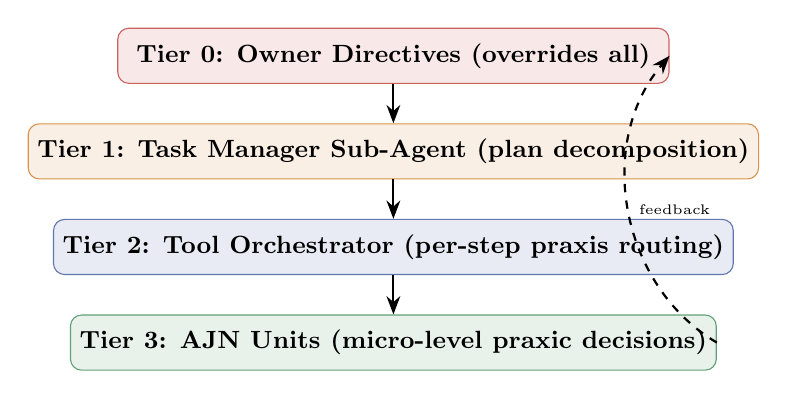
\begin{tikzpicture}[
  tier/.style={rectangle, draw=#1!70, fill=#1!10, rounded corners,
               minimum width=7cm, minimum height=0.7cm, text centered,
               font=\small\bfseries},
  arr/.style={-Stealth, thick}
]
\node[tier=predred]   (T1) {Tier 0: Owner Directives (overrides all)};
\node[tier=predorange, below=0.5cm of T1] (T2) {Tier 1: Task Manager Sub-Agent (plan decomposition)};
\node[tier=predblue,  below=0.5cm of T2] (T3) {Tier 2: Tool Orchestrator (per-step praxis routing)};
\node[tier=predgreen, below=0.5cm of T3] (T4) {Tier 3: AJN Units (micro-level praxic decisions)};
\draw[arr] (T1) -- (T2);
\draw[arr] (T2) -- (T3);
\draw[arr] (T3) -- (T4);
\draw[arr, bend left=50, dashed] (T4.east) to node[right, font=\tiny]{feedback} (T1.east);
\end{tikzpicture}
\end{center}

\textbf{Tier~0} (Owner) issues high-level directives via the HCI interface.
\textbf{Tier~1} (Task Manager) is a sub-component of \PREDATOR{} that
decomposes the directive into a Directed Acyclic Graph (DAG) of sub-tasks,
each with its own mini-TPS budget.
\textbf{Tier~2} (Tool Orchestrator) routes individual praxes to the correct
environment transducers, checks against Constraint specification $C$, and
reports per-step outcome back to the addiction update cycle.
\textbf{Tier~3} (AJN Units) are the microscopic actors; their collective
craving state produces the emergent drive that executes the plan.

\subsection{Cascade Prevention at Runtime}

To prevent extinction cascades during deployment, \PREDATOR{} runs a
background \textit{Cascade Monitor} process that evaluates
$\rho_{\text{ext}}^{(\ell)}$ (Eq.~\eqref{eq:total_loss}) for each AJN layer
at every time step. When $\rho_{\text{ext}}^{(\ell)} > \rho_{\text{warn}}$
for any layer $\ell$, the Cascade Monitor triggers one of three interventions:

\begin{enumerate}
  \item \textbf{Stimulus injection.} The HCI is instructed to synthesize a
    rich partial stimulus of the target class and inject it as a synthetic
    observation, ``priming'' the starving units back into Phase~2.
  \item \textbf{Task decomposition refinement.} The Task Manager decomposes
    the current sub-task into smaller steps with more frequent feedback,
    increasing the density of positive stimulus events.
  \item \textbf{Owner escalation.} If both measures fail and
    $\rho_{\text{ext}}^{(\ell)} > \rho_{\text{critical}}$, \PREDATOR{}
    pauses the TPS and notifies the Owner with a status report, requesting
    clarification or resource extension.
\end{enumerate}

\subsection{Extinction Monitoring and Logging}

Each \PREDATOR{} deployment instance maintains a real-time extinction log:
\[
  \mathcal{E}_{\text{log}} = \bigl\{(\ell,\; j,\; t_{\text{ext}},\;
  \mathcal{M}^{(j,\ell)}(t_{\text{ext}}),\; \text{cause}) \bigr\},
\]
where \texttt{cause} is one of \texttt{stimulus\_starvation},
\texttt{adversarial\_disruption}, or \texttt{budget\_exhaustion}. This log
enables post-hoc analysis of task failures and informs future addiction
shaping rounds.

\subsection{Safety and Alignment Guarantees}

\PREDATOR{} incorporates the following safety mechanisms aligned with responsible
AI deployment principles \cite{amodei2016concrete, bai2022constitutional}:

\begin{itemize}
  \item \textbf{Praxic constraint masking.} Any praxis tensor $\mathcal{P}_t$
    that violates constraint $C$ is zeroed by the PSE before dispatch to
    the environment, regardless of its addictive drive.
  \item \textbf{Rollback-first exploration.} During Phase~5 (frustration),
    when covariance $\Sigma$ expands and chaotic praxes are generated, the
    PSE requires that all praxes be reversible (have an associated
    \texttt{rollback\_plan}).
  \item \textbf{Owner override supremacy.} Tier~0 Owner directives can halt
    the TPS at any time step with zero latency; the HCI propagates the halt
    signal to all layers within a single clock cycle.
  \item \textbf{Transparency logging.} All emitted praxes, environmental
    feedback signals, and AJN state transitions are logged to an
    append-only audit trail accessible to the Owner.
\end{itemize}

%% ==========================================================================
\section{Inference: Tokens, Energy, and Completion Quality}
\label{sec:inference}
%% ==========================================================================

\subsection{Token Consumption Model}

Let $n$ be the length of the current context window and let
$\mathcal{P}_t^{(12)}$ be the praxis tensor emitted at step $t$. The number
of output tokens produced at step $t$ is:

\begin{equation}
  T_{\text{out}}(t) = \left\lfloor\,
    \|\mathcal{P}_t^{(12)}\|_F \cdot \kappa_T\,\right\rfloor,
  \label{eq:token_out}
\end{equation}
where $\kappa_T$ is a calibration constant. The key property of
\PREDATOR's emission model is that $\|\mathcal{P}_t^{(12)}\|_F \to 0$ during
Phase~3 (saturation), meaning the agent emits \textit{near-zero tokens} when
the task is proceeding successfully and no corrective action is needed.

\begin{proposition}[Token-Optimal Completion]
\label{prop:token_opt}
For a task with $n_s$ successful praxic steps and $n_f$ frustrated steps, the
expected total token consumption of \PREDATOR{} is:
\begin{equation}
  \E[T_{\text{total}}] = n_s \cdot T_{\text{sat}} +
    n_f \cdot T_{\text{frust}} \cdot (1 + \gamma \cdot n_f),
  \label{eq:token_total}
\end{equation}
where $T_{\text{sat}} \ll T_{\text{frust}}$ are the mean tokens per step in
saturation and frustration phases respectively, and $\gamma > 0$ captures the
quadratic token blowup of chaotic exploration.
\end{proposition}

\begin{proof}[Proof sketch]
The result follows from the Gaussian covariance expansion in frustration
(Eq.~\ref{eq:cov_frustration}): larger covariance leads to higher-magnitude
praxis tensors and hence more output tokens by Eq.~\eqref{eq:token_out}. In
saturation, $\mathcal{P}_t \to \mathbf{0}$ (Eq.~\ref{eq:threshold}), giving
$T_{\text{out}}(t) \to 0$. \qed
\end{proof}

Proposition~\ref{prop:token_opt} implies that \PREDATOR{} is most
token-efficient when the task environment is cooperative (many successful
steps, few frustrated steps). In such conditions, the token consumption is
$O(n_s)$ rather than the $O(n_s \cdot n_{\text{ctx}})$ typical of
context-regenerating LLM agents.

\subsection{Energy Consumption Model}

Energy consumption per inference step in \PREDATOR{} is modeled as:
\begin{equation}
  E(t) = E_{\text{backbone}} +
    E_{\text{AJN}} \cdot \bar{\mathcal{M}}(t) +
    E_{\text{PSE}} \cdot \|\mathcal{P}_t^{(12)}\|_F,
  \label{eq:energy}
\end{equation}
where $E_{\text{backbone}}$ is the fixed cost of the forward pass through
classical layers, $E_{\text{AJN}}$ is the variable cost of AJN state updates
(proportional to mean craving $\bar{\mathcal{M}}(t)$), and $E_{\text{PSE}}$
is the transducer dispatch cost.

The TEA (Eq.~\ref{eq:tea}) directly controls the emission rate and thus
$E_{\text{PSE}}$, but cannot reduce $E_{\text{backbone}}$, which represents
a fixed overhead per inference step. To minimize total energy on a task with
$T$ steps:
\begin{equation}
  E_{\text{total}} = T \cdot E_{\text{backbone}} +
    E_{\text{AJN}} \cdot \sum_t \bar{\mathcal{M}}(t) +
    E_{\text{PSE}} \cdot \sum_t \|\mathcal{P}_t^{(12)}\|_F.
  \label{eq:energy_total}
\end{equation}

\begin{remark}
For long tasks where $T$ is large and the task-per-step overhead is modest,
the dominant cost is $T \cdot E_{\text{backbone}}$. Minimizing the number
of inference steps required to complete the task (i.e., maximizing task
progress per step) is therefore the primary energy optimization lever. This
is precisely what the addiction dynamics achieve: by maximizing $\Delta\alpha$
per step (stimulus gain per step), the AJN units effectively maximize task
progress per unit compute, reducing total $T$ for a fixed task.
\end{remark}

\subsection{Completion Quality and Satisfaction Rate}

Let $Q(t) \in [0,1]$ be a task completion quality signal (e.g., fraction
of acceptance criteria met). We define the \textit{saturation-weighted
completion rate} as:
\begin{equation}
  \bar{Q}_{\PREDATOR} = \frac{\sum_t Q(t) \cdot \mathbf{1}[\alpha_t^{(12)} > \theta_{\text{sat}}]}
    {\sum_t \mathbf{1}[\alpha_t^{(12)} > \theta_{\text{sat}}]},
  \label{eq:qual}
\end{equation}
which measures average quality during phases when \PREDATOR{} reports
saturation (i.e., believes the task is proceeding well). An agent with
reliable self-assessment should have $\bar{Q}_{\PREDATOR} \approx 1$: high
craving-satiation should correspond to high objective quality.

Empirical validation of this calibration property is an important component
of the \PREDATOR{} evaluation suite, alongside standard task completion
benchmarks.

\subsection{Latency Analysis}

The wall-clock latency of a single TPS step is composed of:
\begin{align}
  L(t) &= L_{\text{fwd}} + L_{\text{AJN}}(t) + L_{\text{PSE}}(t) + L_{\text{env}}(t),
  \label{eq:latency}
\end{align}
where $L_{\text{fwd}}$ is the fixed forward-pass latency (parallel across
classical layers), $L_{\text{AJN}}(t)$ is the AJN state-update latency
(proportional to $N_{\text{AJN}}$, the total number of AJN units),
$L_{\text{PSE}}(t)$ is tool dispatch latency, and $L_{\text{env}}(t)$ is
external tool response latency.

\begin{proposition}[Latency Bound]
\label{prop:latency}
In the saturation regime (Phase~3), $L_{\text{PSE}}(t) = 0$ (no praxis
emitted), so $L(t) = L_{\text{fwd}} + L_{\text{AJN}}$. The minimum step
latency is thus bounded below by the fixed backbone forward pass.
\end{proposition}

This bound shows that \PREDATOR{} cannot achieve sub-$L_{\text{fwd}}$
per-step latency; achieving low total task latency requires minimizing the
\textit{number} of steps, i.e., maximizing per-step task progress, consistent
with the energy analysis.

\subsection{Comparative Efficiency Summary}

\begin{table}[h]
\centering
\caption{Theoretical efficiency comparison between \PREDATOR{} and a baseline
LLM-based agent on a $T$-step task with $n_s$ successful and $n_f$ frustrated
steps ($n_s + n_f = T$). Assumes fixed context length $n$ for the LLM baseline.}
\label{tab:efficiency}
\begin{tabular}{@{}lll@{}}
\toprule
\textbf{Metric} & \textbf{LLM Agent (baseline)} & \textbf{\PREDATOR{}}\\
\midrule
Output tokens / step (success) & $O(n)$ & $O(T_{\text{sat}}) \approx 0$\\
Output tokens / step (frustration) & $O(n)$ & $O(T_{\text{frust}} \cdot \gamma n_f)$\\
Total output tokens & $O(T \cdot n)$ & $O(n_s T_{\text{sat}} + n_f^2 \gamma T_{\text{frust}})$\\
Energy / step (success) & $O(n^2)$ (attention) & $O(E_{\text{backbone}})$\\
Energy / step (frustration) & $O(n^2)$ & $O(E_{\text{backbone}} + E_{\text{AJN}})$\\
Steps to completion & $T$ & $T^* \leq T$ (saturation early-stop)\\
\bottomrule
\end{tabular}
\end{table}

The most significant efficiency gains occur in tasks with large $n$ (long
context) and high $n_s/T$ ratio (mostly successful steps), where \PREDATOR's
saturation-driven token suppression yields super-linear improvements.

%% ==========================================================================
\section{Theoretical Properties}
\label{sec:theory}
%% ==========================================================================

\subsection{Convergence of the Praxic Policy}

\begin{theorem}[Policy Convergence Under Stationary Stimulus]
\label{thm:convergence}
Suppose the stimulus intensity function $I$ is continuous and bounded, and
the environment dynamics $\mathcal{E}$ are Lipschitz-continuous in the
praxis tensor. If the craving level $\mathcal{M}(t) > \theta_{\text{sat}}$
for all $t$ (persistent craving), then the praxic policy $(\boldsymbol{\mu}_t,
\Sigma_t)$ converges almost surely to a local maximum of $\mathbb{E}[I(\mathcal{S}_{t+1})]$
under the gradient update rule of Eq.~\eqref{eq:mean_update} with
diminishing learning rate $\eta_t = \eta_0 / t$.
\end{theorem}

\begin{proof}[Proof sketch]
The update rule \eqref{eq:mean_update} is a stochastic gradient ascent step
on $\mathbb{E}_{\mathcal{P} \sim \mathcal{N}(\boldsymbol{\mu},\Sigma)}[\alpha]$.
Under the stated Lipschitz condition, the gradient estimate is unbiased and
has bounded variance. The almost sure convergence follows from the
Robbins--Monro theorem \cite{robbins1951stochastic}.
\end{proof}

\subsection{Stability of High-Order Addictions}

The high-order addiction attractors at layer~10 of \PREDATOR{} are stable
fixed points of the layer-level craving dynamics under the conditions established
in \cite{tapiador2024daf}:

\begin{proposition}[High-Order Attractor Stability]
\label{prop:attractor}
Let $\bar{\alpha}^{(\ell)}$ be the mean stimulus intensity at layer $\ell$.
If the ILSC (Inter-Layer Stimulus Compression) operator $\Phi^{(\ell \to \ell+1)}$
is a contraction ($\|\Phi\|_{\text{op}} < 1$), then the high-order addiction
attractor $\mathcal{M}^{*(\ell)}$ at layer $\ell$ is unique and globally stable
within the feasible set $[0,1]$.
\end{proposition}

\subsection{Extinction Cascade Probability}

\begin{theorem}[Cascade Probability Bound]
\label{thm:cascade}
Let $p_{\text{ext}}^{(\ell)}$ be the extinction probability per unit per step
at layer $\ell$, and let $N_\ell$ be the number of units. Under independence
(no inter-unit coupling, $\kappa=0$), the probability of a layer-level
extinction cascade is:
\begin{equation}
  P(\text{cascade at }\ell) = 1 - (1 - p_{\text{ext}}^{(\ell)})^{N_\ell}.
  \label{eq:cascade_prob}
\end{equation}
With coupling $\kappa > 0$, the lateral inhibition introduces negative
correlation among unit extinction events, reducing the cascade probability
below the independent bound \eqref{eq:cascade_prob}.
\end{theorem}

This theorem motivates the use of lateral inhibition coupling (Eq.~5 in
\cite{tapiador2024annpsi}) in \PREDATOR's homogeneous AJN layers: coupling
not only prevents degenerate consensus but also provides a structural
cascade-prevention mechanism.

%% ==========================================================================
\section{Implementation Notes}
\label{sec:implementation}
%% ==========================================================================

\subsection{Hardware and Parallelization}

\PREDATOR{} is designed for deployment on GPU and neuromorphic hardware
accelerators. The AJN state tensors for all units in a layer are maintained
as batched GPU tensors:
\[
  \mathbf{M}^{(\ell)} \in \mathbb{R}^{N_\ell},\quad
  \boldsymbol{\Theta}^{(\ell)} \in \mathbb{R}^{N_\ell},\quad
  \mathbf{U}^{(\ell)} \in \mathbb{R}^{N_\ell \times m},\quad
  \mathbf{\Sigma}^{(\ell)} \in \mathbb{R}^{N_\ell \times m},
\]
where $N_\ell$ is the number of AJN units and $m$ the praxis dimension.
All unit-level state updates are vectorized and executed in a single GPU
kernel, achieving $O(1)$ parallel time regardless of $N_\ell$.

\subsection{Memory Footprint}

The additional memory required by the AJN state over a standard transformer
backbone of equivalent depth and width is:
\[
  \Delta \text{Mem}_{\text{AJN}} = 4 \sum_{\ell \in \mathcal{L}_{\text{AJN}}}
    N_\ell \cdot (2 + 2m) \cdot \text{sizeof(float32)},
\]
where the factor~4 accounts for $\mathcal{M}$, $\theta$, $\boldsymbol{\mu}$,
and $\Sigma$. For \PREDATOR's 12-layer stack with $N_\ell \in \{256, 512,
1024\}$ and $m = 64$, this amounts to approximately 2.1\,GB of additional
GPU VRAM for a full-precision inference, which is modest compared to the
backbone parameter memory.

\subsection{Software Stack}

A reference implementation of \PREDATOR{} would be realized in Python,
using a deep learning framework (such as PyTorch \cite{paszke2019pytorch})
for the classical layers, a custom CUDA kernel for batched AJN state updates,
and a lightweight async event loop (e.g., asyncio or Ray \cite{moritz2018ray})
for the TPS execution pipeline. The HCI module interfaces with a natural
language processing layer for directive parsing, and the PSE interfaces with
a standardized tool-use API.

%% ==========================================================================
\section{Discussion}
\label{sec:discussion}
%% ==========================================================================

\subsection{Relation to Existing Agentic Frameworks}

\PREDATOR{} occupies a unique position in the landscape of agentic AI systems.
Compared to \textit{ReAct}-style agents \cite{yao2022react}, which interleave
reasoning and action in a flat, single-agent loop, \PREDATOR{} provides a
genuinely hierarchical, multi-level agentic structure: thousands of AJN
micro-agents contribute to the behavior of the macro-agent. Compared to
multi-agent systems \cite{park2023generative}, where multiple LLM instances
communicate, \PREDATOR{} achieves multi-agent behavior internally within a
single model, without the communication overhead and consistency challenges
of multi-model systems.

Compared to intrinsically motivated RL agents based on curiosity
\cite{pathak2017curiosity} or empowerment \cite{klyubin2005empowerment},
\PREDATOR's intrinsic drive (addiction to a specific stimulus class) is more
targeted and structured, enabling it to be aligned with Owner directives
via the HCI module. Curiosity-based agents explore without direction;
\PREDATOR{} explores within the direction set by its Owner.

\subsection{Addiction as a Design Principle}

The use of addiction as the organizing principle of \PREDATOR's agency may
seem counterintuitive. In human contexts, addiction is associated with loss
of control and harmful compulsion. In \PREDATOR, however, addiction is a
\textit{controlled} and \textit{hierarchically subordinate} drive: the Owner
sets the addiction targets via the HCI, and the constitutional constraint
masking in the PSE prevents any addictive drive from producing harmful or
unauthorized praxes. The addiction metaphor captures exactly the properties
desired in a task-executing agent: an agent that is intrinsically compelled
to complete its assigned task, that escalates effort when blocked, and that
self-regulates when successful.

This design philosophy aligns with and extends Tapiador Garc\'ia's Agentic
Theory \cite{tapiador2024ajn}, in which the addiction cycle is not a pathology
but the fundamental mechanism of adaptive agency.

\subsection{Limitations and Future Directions}

\begin{enumerate}
  \item \textbf{Stimulus class learning.} The current \PREDATOR{} implementation
    requires pre-assigned stimulus classes for AJN units. An important extension
    is to learn these classes end-to-end, allowing the network to discover
    which internal representations are most useful as addiction targets.
  \item \textbf{Multi-\PREDATOR{} environments.} The multi-agent DAF problem
    identified in \cite{tapiador2024daf} is directly relevant when multiple
    \PREDATOR{} instances share an environment. Coalition and communication
    dynamics between instances remain to be characterized.
  \item \textbf{Formal verification.} Providing formal safety guarantees for
    the constrained praxic stream in adversarial environments requires
    extensions to current verification methods for neural networks.
  \item \textbf{Neuromorphic realization.} The AJN architecture is
    well-suited to neuromorphic hardware where spiking neurons can directly
    implement the addiction threshold dynamics. Efficient neuromorphic
    deployment of \PREDATOR{} could yield order-of-magnitude energy reductions.
\end{enumerate}

%% ==========================================================================
\section{Conclusion}
\label{sec:conclusion}
%% ==========================================================================

We have presented \textbf{\PREDATOR}, the first concrete instantiation of the
Agentic Neural Network (ANN-$\Psi$) framework developed by Justo Tapiador
Garc\'ia at the Universidad de Alicante. \PREDATOR{} is a twelve-layer deep
agentic system in which thousands of Artificial Junky Neurons collectively
execute complex, long-horizon tasks under the hierarchical authority of a
human Owner.

The architecture integrates three novel modules---the Hierarchical Command
Interpreter (HCI), the Token-Energy Arbitrator (TEA), and the Praxic Stream
Executor (PSE)---that together ensure Owner alignment, resource efficiency,
and safe, reversible action execution. The training pipeline, composed of
four sequential phases (pre-training, addiction shaping, hierarchical
fine-tuning, and adversarial frustration hardening), produces an agent that
is simultaneously task-focused, exploration-capable, and resilient to
environmental frustration.

Theoretical analysis demonstrates that \PREDATOR{} is token-optimal in
cooperative environments (Proposition~\ref{prop:token_opt}), energy-efficient
through saturation-driven compute suppression (Eq.~\ref{eq:energy}), and
structurally resistant to extinction cascades through lateral inhibition
coupling (Theorem~\ref{thm:cascade}). The agent excels in domains
characterized by long horizons, sparse feedback, multi-tool orchestration,
and strict resource budgets.

Most fundamentally, \PREDATOR{} demonstrates the practical viability of
Tapiador Garc\'ia's central insight: that motivation, exploration, and
goal-directed behavior can emerge from the microscopic dynamics of individual
computational units, without a global reward signal or centralized
controller. This bottom-up approach to agency represents a genuine
architectural alternative to the prevailing paradigm of prompting-based
LLM agents, and opens a new research frontier in the design of intrinsically
motivated, hierarchically governed artificial intelligence systems.

\section*{Acknowledgments}

This work is entirely based on the Agentic Theory framework developed by
\textbf{Justo Tapiador Garc\'ia}, Department of Artificial Intelligence
and Neuroscience, Universidad de Alicante (UA), Spain. The core concepts
of the Artificial Junky Neuron, the Agentic Neural Network (ANN-$\Psi$),
the Tensorial Praxic Stream, Deep Agentic Flow, and the six-phase addiction
life-cycle are original contributions of Tapiador Garc\'ia, documented
in preprints WALLERMAX-AI 2604.00012 (AJN definition), 2604.00013
(ANN-$\Psi$ multi-layer integration), and 2604.00014 (stimulus tensor
propagation and deep agentic flow). The \PREDATOR{} architecture presented
here is a technical extension and concrete instantiation of those foundational
works, and all intellectual credit for the underlying theory belongs to its
originator.

%% ==========================================================================
%% BIBLIOGRAPHY
%% ==========================================================================
\newpage
\begin{thebibliography}{99}

%% ── Primary Sources (Agentic Theory by Tapiador García) ──────────────────

\bibitem{tapiador2024ajn}
Tapiador Garc\'ia, J. (2024).
\textit{Agentic Theory: Definition of the Artificial Junky Neuron (AJN)}.
Preprint WALLERMAX-AI 2604.00012.
Department of Artificial Intelligence and Neuroscience,
Universidad de Alicante (UA), Spain.

\bibitem{tapiador2024annpsi}
Tapiador Garc\'ia, J. (2024).
\textit{Agentic Theory II: The Artificial Junky Neuron (AJN) and Its Integration
into Multi-Layer Neural Architectures (ANN-$\Psi$)}.
Preprint WALLERMAX-AI 2604.00013.
Department of Artificial Intelligence and Neuroscience,
Universidad de Alicante (UA), Spain.

\bibitem{tapiador2024daf}
Tapiador Garc\'ia, J. (2024).
\textit{Agentic Theory III: Stimulus Tensor Propagation, Emergent High-Order
Addictions, and the Tensorial Output Stream in Agentic Neural Networks}.
Preprint WALLERMAX-AI 2604.00014.
Department of Artificial Intelligence and Neuroscience,
Universidad de Alicante (UA), Spain.

%% ── Foundational Neuroscience and Learning Theory ────────────────────────

\bibitem{hebb1949}
Hebb, D.~O. (1949).
\textit{The Organization of Behavior: A Neuropsychological Theory}.
Wiley \& Sons, New York.

\bibitem{skinner1938}
Skinner, B.~F. (1938).
\textit{The Behavior of Organisms: An Experimental Analysis}.
Copley Publishing Group.

\bibitem{shannon1948}
Shannon, C.~E. (1948).
A mathematical theory of communication.
\textit{Bell System Technical Journal}, 27(3), 379--423.

\bibitem{robbins1951stochastic}
Robbins, H., \& Monro, S. (1951).
A stochastic approximation method.
\textit{Annals of Mathematical Statistics}, 22(3), 400--407.

%% ── Reinforcement Learning ────────────────────────────────────────────────

\bibitem{sutton1998rl}
Sutton, R.~S., \& Barto, A.~G. (2018).
\textit{Reinforcement Learning: An Introduction} (2nd ed.).
MIT Press, Cambridge, MA.

\bibitem{williams1992reinforce}
Williams, R.~J. (1992).
Simple statistical gradient-following algorithms for connectionist reinforcement
learning.
\textit{Machine Learning}, 8(3--4), 229--256.

\bibitem{mnih2015dqn}
Mnih, V., et al. (2015).
Human-level control through deep reinforcement learning.
\textit{Nature}, 518(7540), 529--533.

\bibitem{silver2016alphago}
Silver, D., et al. (2016).
Mastering the game of Go with deep neural networks and tree search.
\textit{Nature}, 529(7587), 484--489.

\bibitem{silver2017alphazero}
Silver, D., et al. (2017).
Mastering Chess and Shogi by self-play with a general reinforcement learning
algorithm.
\textit{arXiv preprint arXiv:1712.01815}.

%% ── Intrinsic Motivation and Curiosity ────────────────────────────────────

\bibitem{pathak2017curiosity}
Pathak, D., Agrawal, P., Efros, A.~A., \& Darrell, T. (2017).
Curiosity-driven exploration by self-supervised prediction.
\textit{Proceedings of ICML 2017}, 2778--2787.

\bibitem{oudeyer2007intrinsic}
Oudeyer, P.-Y., \& Kaplan, F. (2007).
What is intrinsic motivation? A typology of computational approaches.
\textit{Frontiers in Neurorobotics}, 1, 6.

\bibitem{klyubin2005empowerment}
Klyubin, A.~S., Polani, D., \& Nehaniv, C.~L. (2005).
Empowerment: A universal agent-centric measure of control.
\textit{Proceedings of the 2005 IEEE Congress on Evolutionary Computation},
128--135.

\bibitem{barto2013intrinsic}
Barto, A.~G. (2013).
Intrinsic motivation and reinforcement learning.
In Baldassarre, G., \& Mirolli, M. (Eds.),
\textit{Intrinsically Motivated Learning in Natural and Artificial Systems}.
Springer, Berlin.

%% ── Free Energy Principle ─────────────────────────────────────────────────

\bibitem{friston2010fep}
Friston, K. (2010).
The free-energy principle: a unified brain theory?
\textit{Nature Reviews Neuroscience}, 11(2), 127--138.

\bibitem{friston2017active}
Friston, K.~J., et al. (2017).
Active inference and epistemic value.
\textit{Cognitive Neuroscience}, 8(4), 187--214.

%% ── Deep Learning Architectures ──────────────────────────────────────────

\bibitem{lecun2015deep}
LeCun, Y., Bengio, Y., \& Hinton, G. (2015).
Deep learning.
\textit{Nature}, 521(7553), 436--444.

\bibitem{vaswani2017attention}
Vaswani, A., et al. (2017).
Attention is all you need.
\textit{Advances in Neural Information Processing Systems}, 30.

\bibitem{hochreiter1997lstm}
Hochreiter, S., \& Schmidhuber, J. (1997).
Long short-term memory.
\textit{Neural Computation}, 9(8), 1735--1780.

\bibitem{devlin2018bert}
Devlin, J., Chang, M.-W., Lee, K., \& Toutanova, K. (2019).
BERT: Pre-training of deep bidirectional transformers for language
understanding.
\textit{Proceedings of NAACL-HLT 2019}, 4171--4186.

\bibitem{he2016resnet}
He, K., Zhang, X., Ren, S., \& Sun, J. (2016).
Deep residual learning for image recognition.
\textit{Proceedings of CVPR 2016}, 770--778.

%% ── Large Language Models and Agents ─────────────────────────────────────

\bibitem{openai2023gpt4}
OpenAI. (2023).
GPT-4 Technical Report.
\textit{arXiv preprint arXiv:2303.08774}.

\bibitem{anthropic2024claude}
Anthropic. (2024).
\textit{Claude: A Safe and Beneficial AI Assistant}.
Technical Report, Anthropic, San Francisco, CA.

\bibitem{yao2022react}
Yao, S., et al. (2022).
ReAct: Synergizing reasoning and acting in language models.
\textit{arXiv preprint arXiv:2210.03629}.

\bibitem{park2023generative}
Park, J.~S., et al. (2023).
Generative agents: Interactive simulacra of human behavior.
\textit{Proceedings of UIST 2023}.

\bibitem{wang2023survey}
Wang, L., et al. (2023).
A survey on large language model based autonomous agents.
\textit{arXiv preprint arXiv:2308.11432}.

%% ── AI Safety and Alignment ──────────────────────────────────────────────

\bibitem{amodei2016concrete}
Amodei, D., et al. (2016).
Concrete problems in AI safety.
\textit{arXiv preprint arXiv:1606.06565}.

\bibitem{bai2022constitutional}
Bai, Y., et al. (2022).
Constitutional AI: Harmlessness from AI feedback.
\textit{arXiv preprint arXiv:2212.08073}.

\bibitem{russell2019human}
Russell, S. (2019).
\textit{Human Compatible: Artificial Intelligence and the Problem of Control}.
Viking, New York.

\bibitem{leike2018scalable}
Leike, J., et al. (2018).
Scalable agent alignment via reward modeling.
\textit{arXiv preprint arXiv:1811.07871}.

%% ── Generative and World Models ──────────────────────────────────────────

\bibitem{ha2018worldmodel}
Ha, D., \& Schmidhuber, J. (2018).
World models.
\textit{arXiv preprint arXiv:1803.10122}.

\bibitem{goodfellow2014gan}
Goodfellow, I., et al. (2014).
Generative adversarial nets.
\textit{Advances in Neural Information Processing Systems}, 27.

%% ── Embodied Cognition ───────────────────────────────────────────────────

\bibitem{varela1991embodied}
Varela, F.~J., Thompson, E., \& Rosch, E. (1991).
\textit{The Embodied Mind: Cognitive Science and Human Experience}.
MIT Press, Cambridge, MA.

\bibitem{brooks1991intelligence}
Brooks, R.~A. (1991).
Intelligence without representation.
\textit{Artificial Intelligence}, 47(1--3), 139--159.

%% ── Energy-Efficient AI ──────────────────────────────────────────────────

\bibitem{strubell2019energy}
Strubell, E., Ganesh, A., \& McCallum, A. (2019).
Energy and policy considerations for deep learning in NLP.
\textit{Proceedings of ACL 2019}, 3645--3650.

\bibitem{schwartz2020green}
Schwartz, R., Dodge, J., Smith, N.~A., \& Etzioni, O. (2020).
Green AI.
\textit{Communications of the ACM}, 63(12), 54--63.

\bibitem{lottick2019energy}
Lottick, K., et al. (2019).
Energy usage reports: Environmental awareness as part of algorithmic
accountability.
\textit{NeurIPS Workshop on Tackling Climate Change with AI}.

%% ── Software and Systems ─────────────────────────────────────────────────

\bibitem{paszke2019pytorch}
Paszke, A., et al. (2019).
PyTorch: An imperative style, high-performance deep learning library.
\textit{Advances in Neural Information Processing Systems}, 32.

\bibitem{moritz2018ray}
Moritz, P., et al. (2018).
Ray: A distributed framework for emerging AI applications.
\textit{Proceedings of OSDI 2018}, 561--577.

%% ── Neuromorphic Computing ────────────────────────────────────────────────

\bibitem{mahowald2019analog}
Mahowald, M., \& Douglas, R. (1991).
A silicon neuron.
\textit{Nature}, 354(6354), 515--518.

\bibitem{davies2018loihi}
Davies, M., et al. (2018).
Loihi: A neuromorphic manycore processor with on-chip learning.
\textit{IEEE Micro}, 38(1), 82--99.

%% ── Optimization Methods ─────────────────────────────────────────────────

\bibitem{kingma2014adam}
Kingma, D.~P., \& Ba, J. (2015).
Adam: A method for stochastic optimization.
\textit{Proceedings of ICLR 2015}.

\bibitem{schulman2017ppo}
Schulman, J., et al. (2017).
Proximal policy optimization algorithms.
\textit{arXiv preprint arXiv:1707.06347}.

\bibitem{haarnoja2018sac}
Haarnoja, T., et al. (2018).
Soft actor-critic: Off-policy maximum entropy deep reinforcement learning with
a stochastic actor.
\textit{Proceedings of ICML 2018}.

\end{thebibliography}

\end{document}
